\section{Computational Companion}
\label{sec:ch02-computational-companion}

Computation is most useful here when it makes local geometry visible or checks an analytic calculation. The source files for this section are stored in \texttt{examples/python/ch02/} and \texttt{examples/wolfram/ch02/}.

\subsection{Python: Surfaces, Gradients, and Jacobians}

The complete Python program uses NumPy for array calculations and Matplotlib for visualization. It generates the figures in this section and verifies a numerically approximated Jacobian against its exact analytic form.

\lstinputlisting[style=prbookpython,caption={Python computational companion for Chapter 2.},label={lst:ch02-python}]{examples/python/ch02/differential_calculus_companion.py}

\begin{bookfigure}[H]{A surface plot makes the scalar field $f(x,y)=x^2+\tfrac12y^2$ visible as a geometric object.}
\label{fig:ch02-computational-surface}
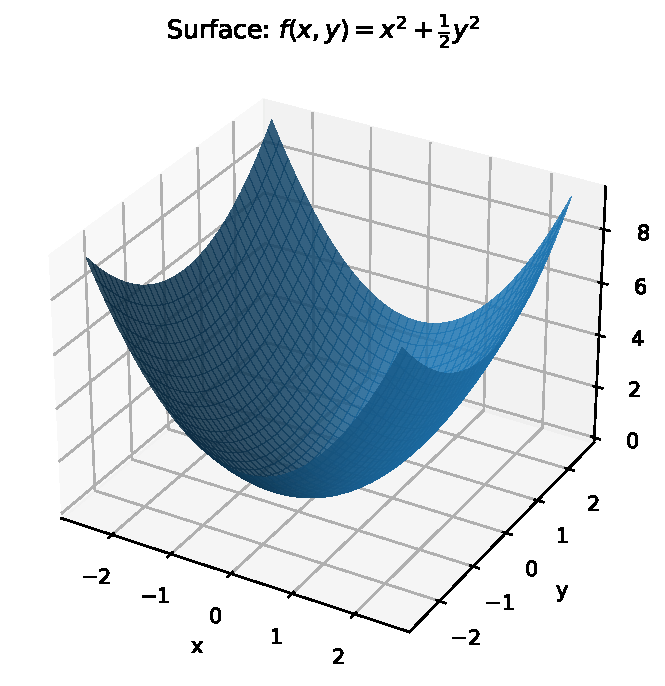
\includegraphics[width=.78\textwidth]{generated/ch02/surface_plot.pdf}
\end{bookfigure}

\begin{bookfigure}[H]{Normalized gradient vectors cross the level curves of $f=x^2+y^2$ orthogonally.}
\label{fig:ch02-computational-gradient}
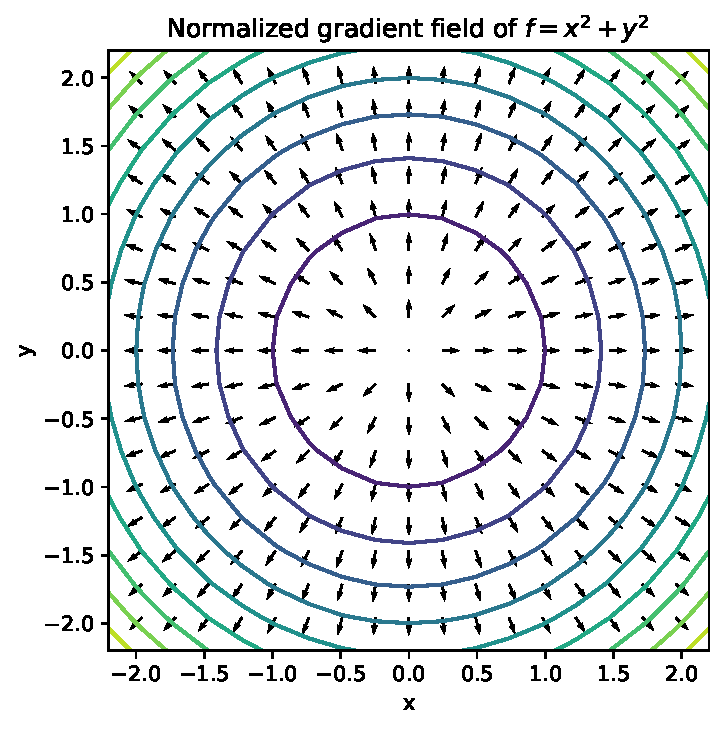
\includegraphics[width=.72\textwidth]{generated/ch02/gradient_field.pdf}
\end{bookfigure}

\begin{bookfigure}[H]{A nonlinear map deforms a rectangular parameter grid. The Jacobian at each point is the best local linear description of that deformation.}
\label{fig:ch02-computational-jacobian}
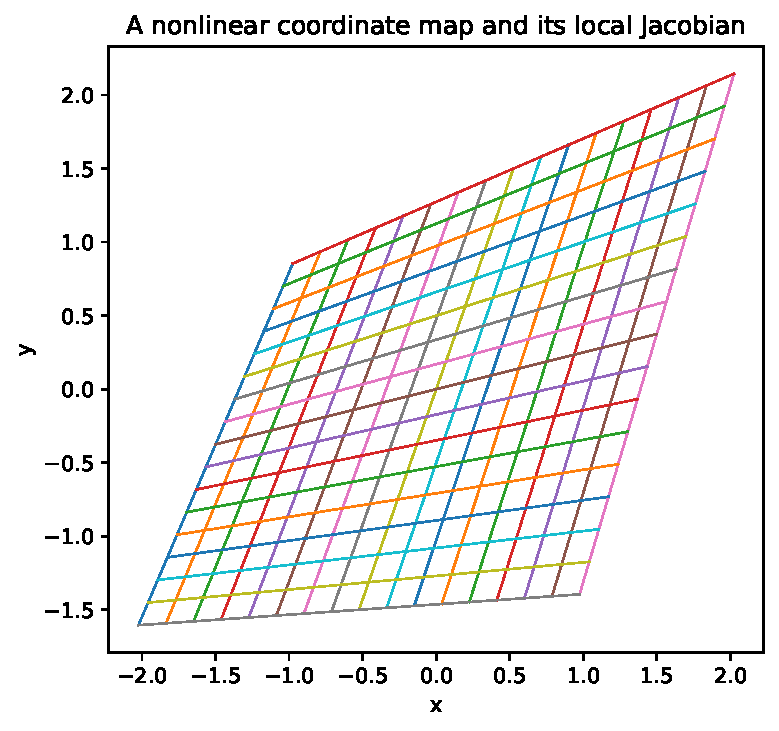
\includegraphics[width=.74\textwidth]{generated/ch02/jacobian_grid.pdf}
\end{bookfigure}

\begin{bookfigure}[H]{For a fixed gradient, the directional derivative varies sinusoidally with direction and is bounded by $\pm\lVert\nabla f\rVert$.}
\label{fig:ch02-computational-directional}
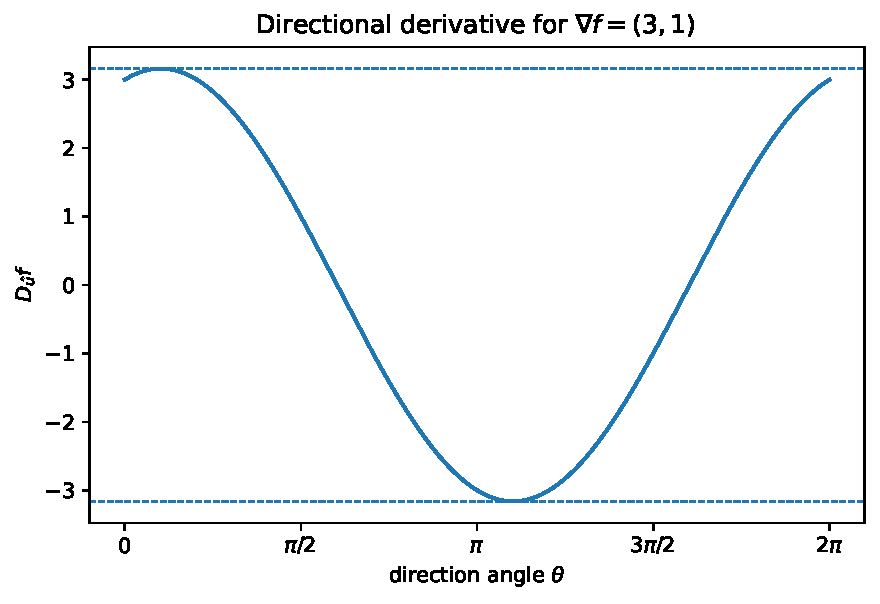
\includegraphics[width=.78\textwidth]{generated/ch02/directional_derivative.pdf}
\end{bookfigure}

\begin{bookinsight}[Numerical differentiation]
A centered finite difference usually has smaller truncation error than a forward difference. Nevertheless, numerical derivatives depend on the step size: a step that is too large produces truncation error, while a step that is too small magnifies floating-point cancellation. Analytic derivatives remain the reference whenever they are available.
\end{bookinsight}

\subsection{Wolfram Language: Symbolic and Visual Checks}

The Wolfram Language companion differentiates symbolically, computes gradients and Hessians, plots scalar and vector fields, and evaluates a Jacobian determinant.

\lstinputlisting[style=prbookwolfram,caption={Wolfram Language companion for Chapter 2.},label={lst:ch02-wolfram}]{examples/wolfram/ch02/differential_calculus_companion.wl}

\begin{mistakebox}[A plot is not a proof]
A plot may suggest continuity, differentiability, or the location of an extremum, but it cannot establish these properties by itself. Sampling can miss singularities or narrow features. Use visualization to form and test intuition, then use definitions and analysis to justify the conclusion.
\end{mistakebox}
